\documentclass[journal,12pt,twocolumn]{IEEEtran}
\usepackage{graphicx}
\usepackage[margin=0.5in]{geometry}
\usepackage[cmex10]{amsmath}
\usepackage{array}
\usepackage{booktabs}
\usepackage{mathtools}
\usepackage{hyperref}


\title{\textbf{Optimization Assignment - 1}}
\author{kanekal kousar}
\date{September 2022}


\providecommand{\norm}[1]{\left\lVert#1\right\rVert}
\providecommand{\abs}[1]{\left\vert#1\right\vert}
\let\vec\mathbf
\newcommand{\myvec}[1]{\ensuremath{\begin{pmatrix}#1\end{pmatrix}}}
\newcommand{\mydet}[1]{\ensuremath{\begin{vmatrix}#1\end{vmatrix}}}
\providecommand{\brak}[1]{\ensuremath{\left(#1\right)}}
\providecommand{\lbrak}[1]{\ensuremath{\left(#1\right.}}
\providecommand{\rbrak}[1]{\ensuremath{\left.#1\right)}}
\providecommand{\sbrak}[1]{\ensuremath{{}\left[#1\right]}}

\begin{document}
\maketitle

\section{Question}
\textbf{-Investigate for the maxima and minima of the function
 $f(x)=\int_{1}^{x}2(t-1)(t-3)^3+3(t-1)^2(t-2)^2 \,dx$}
 
 \section{Solution}
 \textbf{STEP-1}
 The given function \textbf{f(x)} can be written as
 \begin{align}
 f(x)=(x-2)^3(x-1)^2
 \end{align}
 \textbf{STEP-2}
 we can find the maxima of eq(1) by using gradient ascent method
 
$\implies x_{n+1} = x_n + \alpha \nabla f(x_n) $\\
 \begin{align}
        \implies x_{n+1} &= x_n + \alpha \brak{(x_n-1)(x_n-2)^2(5x_n-7)}
    \end{align}
 Taking $x_0=0.5,\alpha=0.001$ and precision = 0.00000001, values obtained using python are:
    
    \begin{align}
        \boxed{\text{Maxima} = -2.4985e^-11}\\
        \boxed{\text{Maxima Point} = 1}
    \end{align}
 
 \textbf{STEP-3}
 we can find the minima of eq(1) by using gradient descent method
 
$\implies x_{n+1} = x_n - \alpha \nabla f(x_n) $\\
 \begin{align}
        \implies x_{n+1} &= x_n - \alpha \brak{(x_n-1)(x_n-2)^2(5x_n-7)}
    \end{align}
Taking $x_0=1.5,\alpha=0.001$ and precision = 0.00000001, values obtained using python are:
    
    \begin{align}
        \boxed{\text{Minima} =-0.03455}\\
        \boxed{\text{Minima Point} = 1.4}
    \end{align}
\begin{figure}[h!]
\centering
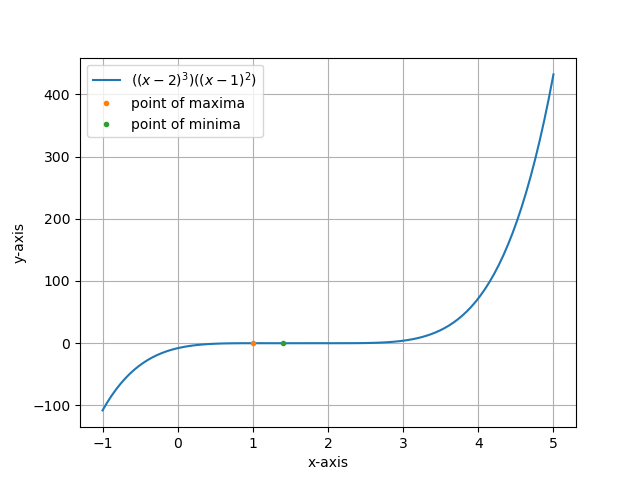
\includegraphics[scale=0.5]{fig/op1.png}  \\
\caption{plot of f(x) with maxima and minima points}
\end{figure}
    
Get the python code of the figures from
\begin{table}[h]
\large
\centering
\framebox{
\url{https://github.com/kkousar/KOUSAR_FWC/blob/main/optimization_1/code/optimization1.py}}
\bibliographystyle{ieeetr}
\end{table}
 
\end{document}